\documentclass[]{article}
\usepackage{ragged2e}
\usepackage{amsmath}
\usepackage{listings}
\usepackage{graphicx}




%opening
\title{Microprocessors ETI 2407 \\
Assignment I}
\author{\textbf{Mugo Mwaura} 
	ENE221-0280/2016}
\date{August 31, 2020\endgraf\rule{\textwidth}{.9pt}}

\begin{document}

\maketitle



\section{Question One}


\justify
Write an assembly program that displays whole numbers and their squares. A user should
input the last number. The output below shows what would happen if a user entered 5. What
is the highest value you could enter that gave correct results? Explain why this number is the
limit and what can be done to improve this limit:


\begin{align*}
x \qquad x^2 \\
1 \qquad 1 \\
2 \qquad 4 \\
3\qquad 9 \\
4 \hspace*{1.5em} 16 \\
5\hspace*{1.5em} 25\\
\end{align*}

\subsection{Answer Explanation}

\textbf{Highest value} entered that gave the correct result is $181$ i.e., $floor\left(\sqrt{\frac{2^{16}}{2}}\right)$.
Highest number giving result = $2^{16}$.
Registers (AX) store 16 bit values. However, if this program was using a signed
representation, the maximum would be:
\begin{equation*}
\frac{2^{16}}{2} = 32,767
\end{equation*}


For a $32 bit$ answer, the result is placed in DX:AX or effectively, if using a single 32 bit register, EAX.
This program does compute the answer upto a max of 65,556 therefore,
but since we are only printing from AX (using \textbf{emu8086 print\_num} procedure), and haven't manually implemented
printing from DX:AX, the maximum result we get is similar to that of a signed value.


\subparagraph{What can be done to improve the limit?}
Print the entire result from EAX for a $2^{16}$ value. Beyond that, we can't go as the addresses
only access $64 KB$ of addressable memory

\subsection{Pseudo-code}
\begin{enumerate}
	\item Get maximum value $x$ from user
	\item initialize loop counter $c$ to $1$
	\item \textbf{while $c $ $<= x$ }
	\begin{itemize}
		\item print $c$
		\item print $c \times c$
		\item \textbf{end loop}
	\end{itemize}
\end{enumerate}

\subsection{Code} \label{script 1}
\lstinputlisting[language=python]{Q_one/q_one.asm}

\clearpage
\subsection{Program Output}

\begin{figure}[h]
	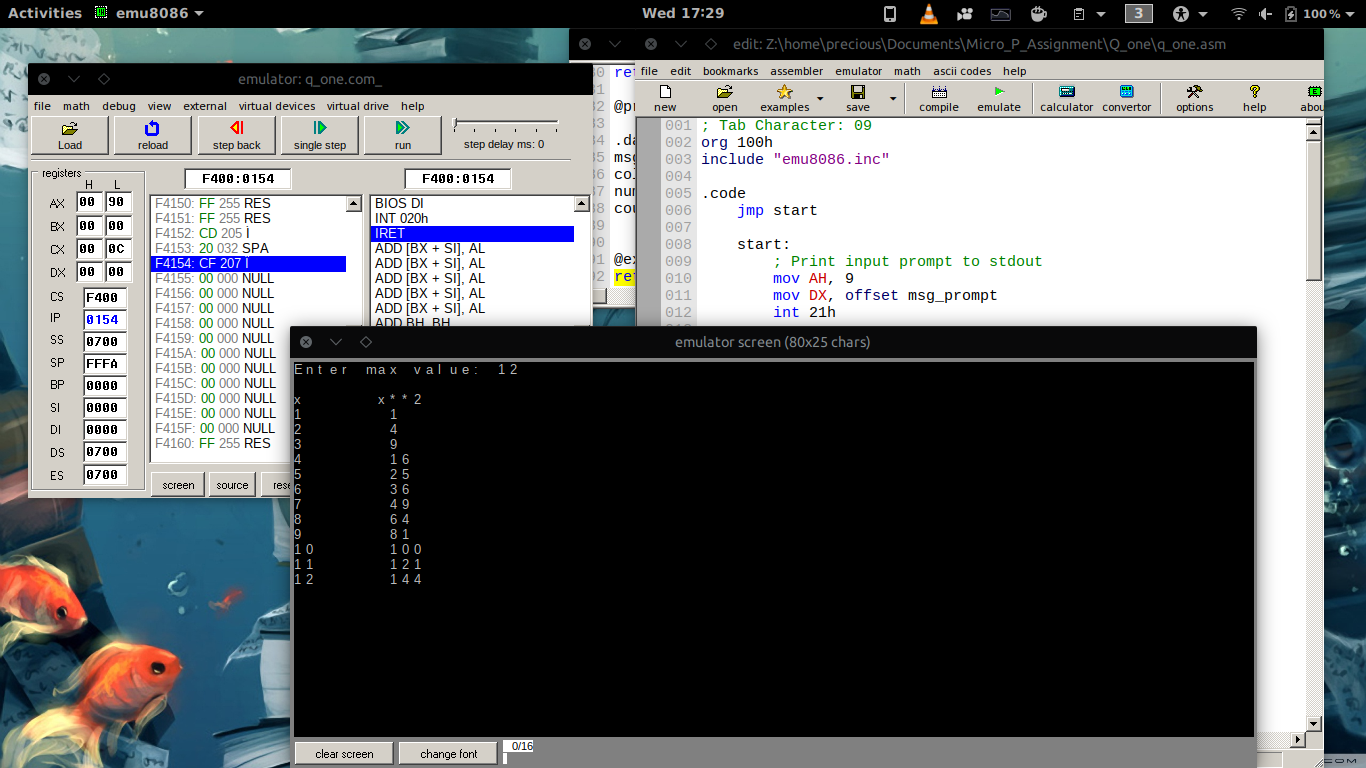
\includegraphics[width=15cm]{Q_one/q1_updated_aug26.png}
	\centering
	\caption{A screenshot of the output from running script \ref{script 1}}
\end{figure}



\newpage
\clearpage
\section{Question Two}
Write a program that allows you convert from a number to the corresponding ASCII value.

\centering
E.g., if a user enters $35$, the output should be $\#$.

\justify
The program should also have a provision
for displaying the ASCII value of an entered character.

\centering
E.g., if a user enters $*$, the output
should be 42.

\justify
At the start of the program, a user should choose the option between the $2$
modes (either ASCII value to character OR character to ASCII value).
NB: Your code should be able to deal with erroneous input appropriately

\centering
E.g. entering a number above $255$.

\justify

\subsection{Psedo-code}

\begin{enumerate}
	\item Select program mode \\
	\hspace*{3em} a) ASCII to Decimal \\
	\hspace*{3em} b) Decimal to ASCII \\
	\item Get input from user $input$
	\begin{itemize}
		\item If mode $(b)$ and input$ >$ $255$, \textbf{error}
	\end{itemize}
	
	\item Initialize ASCII counter $c$. Initialize DEC counter $d$
	
	\item \textbf{Start loop:}
	\begin{itemize}
	\item If $input$ == $ASCII_{i}$, (where $ASCII$ is the set of all ASCII characters) \\
	\hspace*{6em} print $ASCII_i$, print $DEC_i$, (where $DEC$ is an enumeration of the $ASCII$ set) \\
	\textbf{end loop}
	
	\end{itemize}

\end{enumerate}

\subsection{Code} \label{sketch 2}
\lstinputlisting[language=python]{q_two/q_two.asm}

\clearpage
\subsection{Program Output}

\begin{figure}[h]
	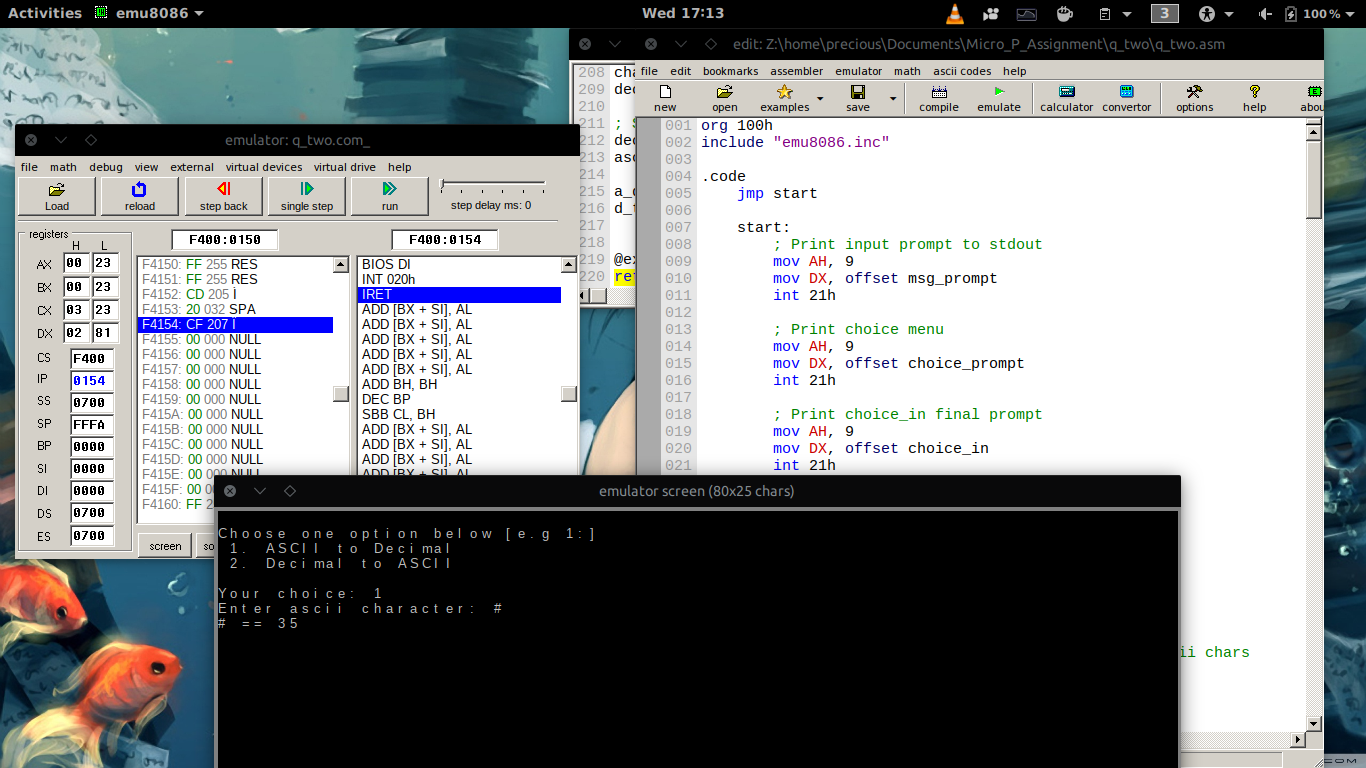
\includegraphics[width=12cm]{q_two/q2_ascii_to_dec.png}
	\centering
	\caption{A screenshot of the output from running script \ref{script 1}. \textbf{Converting ASCII to decimal}}
\end{figure}

\begin{figure}[h]
	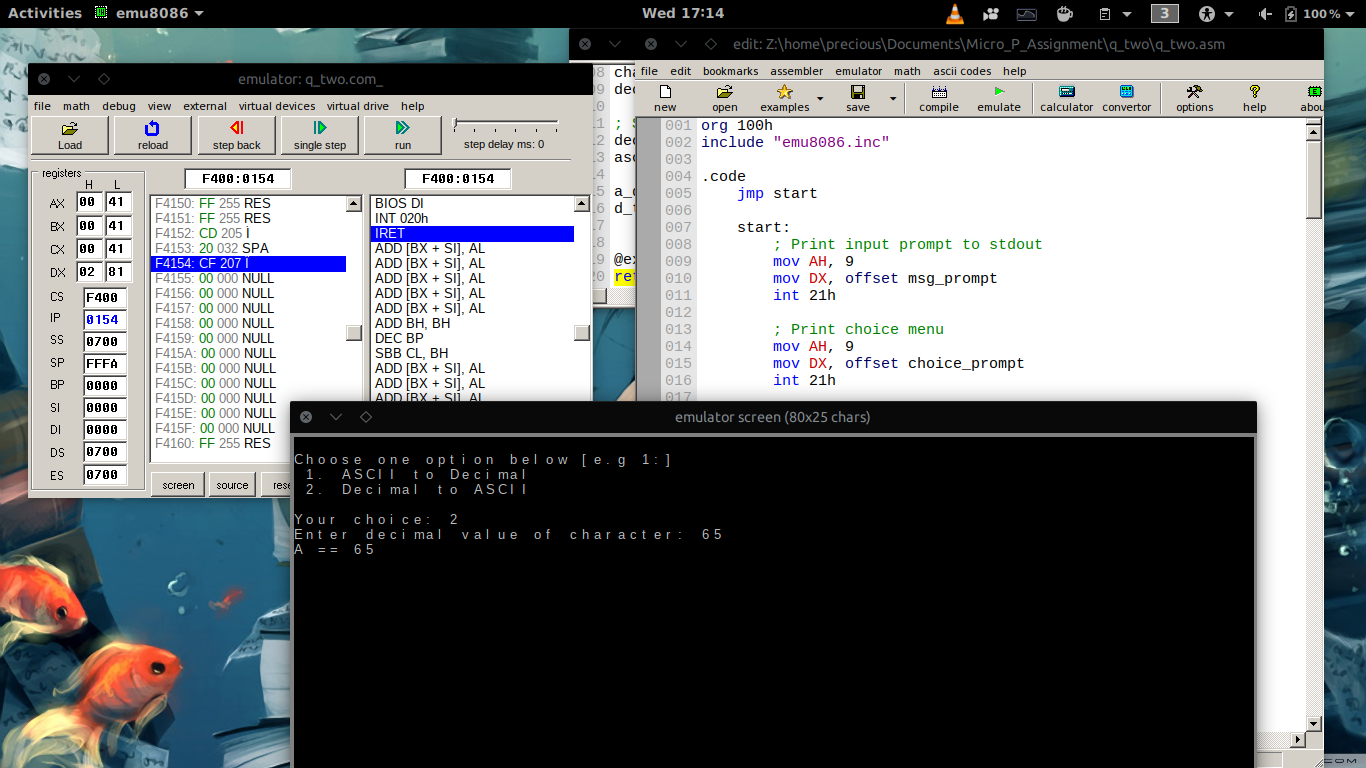
\includegraphics[width=12cm]{q_two/q2_dec_to_ascii.png}
	\centering
	\caption{A screenshot of the output from running script \ref{script 1}. \textbf{Converting decimal to ASCII}}
\end{figure}


\begin{figure}[h]
	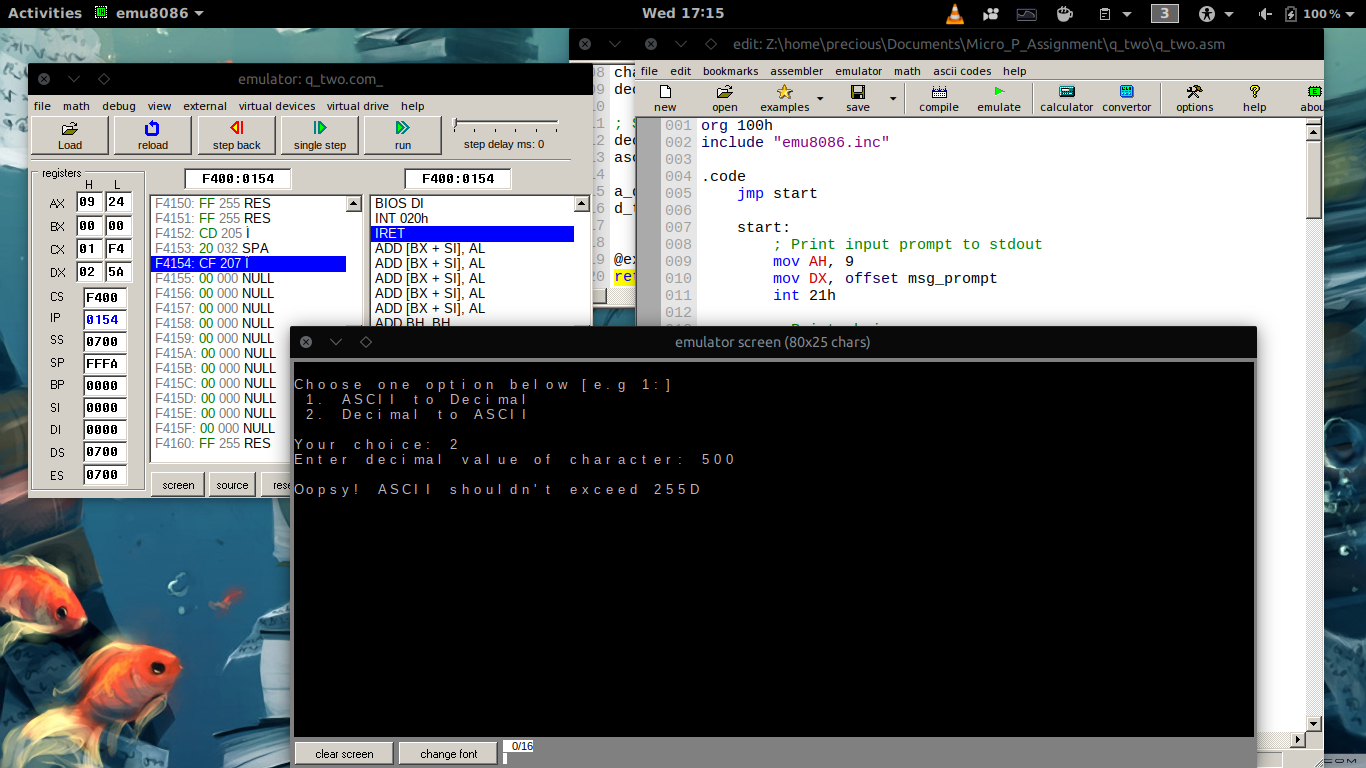
\includegraphics[width=12cm]{q_two/q2_input_gthan_255.png}
	\centering
	\caption{A screenshot of the output from running script \ref{script 1}. \textbf{Error on Decimal value greater that $255$}}
\end{figure}

\clearpage
\section{Question Three}

Develop a virus that changes the letters being typed randomly into other letters and thus frustrates the user. E.g. if he intends to type \emph{Hello boss}, it could instead display something like \emph{Sdupl dwsp}. (For simplicity, assume that the email will be written into your running program. i.e., you do not need to write code for attacking the browser, \textbf{ though if you do that, come get a cookie}).

After writing your code, describe what would happen if a user typed
1234?

\subsection{Answer Explanation}
\textbf{If the user types "\emph{1234?}}" the program will output "1234?" to stdout(See Figure \ref{fig:5}). The program only changes alphabetical ASCII inputs. i.e., $65 - 90 $ and $97 - 122$. The rest of the inputs are printed as keyed in by the user.

\subsection{Pseudo-code}
\begin{enumerate}
	\item \textbf{Loop:}
	\begin{itemize}
		\item (a) Get character $c$ from user without echo
		\item \textbf{If} $c$ is an alphabet: \\
		\hspace*{6em} Alter the value of $c$ randomly
		\item Print the value of $c$
		\item Go back to \textbf{(a)}
		
	\end{itemize}
\end{enumerate}


\subsection{Code} \label{sketch 3}
\lstinputlisting[language=python]{q_three/q_three.asm}

\clearpage
\subsection{Program Output}


\begin{figure}[h]
	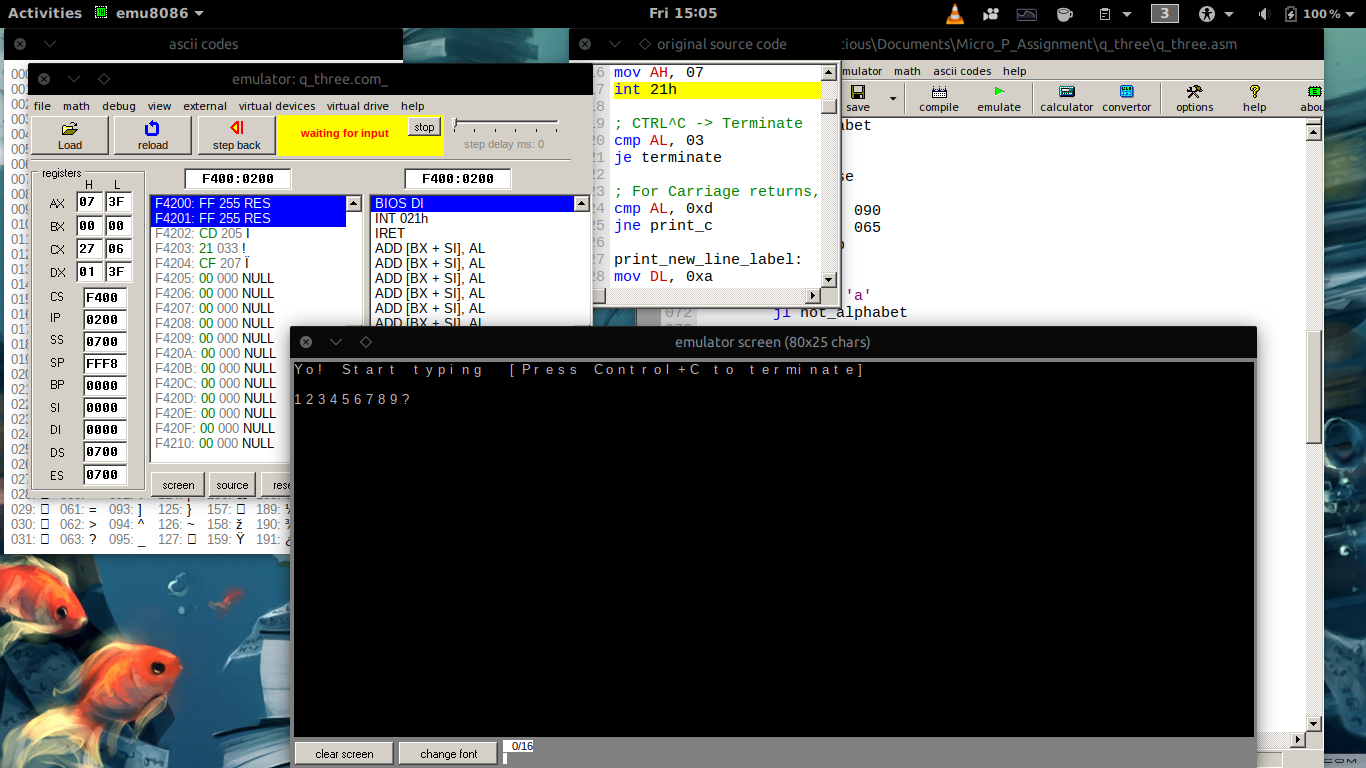
\includegraphics[width=12cm]{q_three/q_3 print 123456789?.png}
	\centering
	\caption{A screenshot of the output from running script \ref{sketch 3}. \textbf{An input of "1234?" outputs "1234?"}}
	\label{fig:5}
\end{figure}


\begin{figure}[h]
	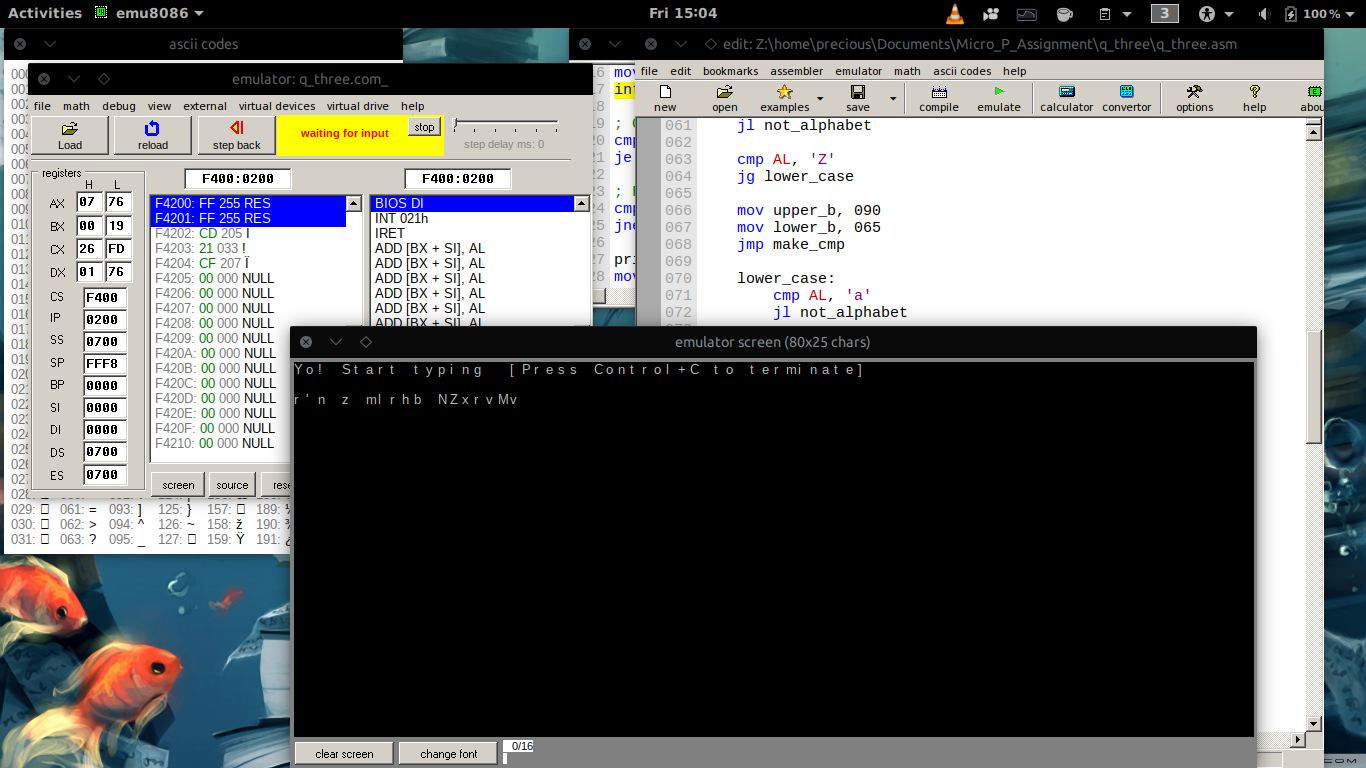
\includegraphics[width=12cm]{q_three/q_3_printing_I'm a noisy machine.png}
	\centering
	\caption{A screenshot of the output from running script \ref{sketch 3}. \textbf{The output of the input "I'm a noisy machine"}}
\end{figure}


\begin{figure}[h]
	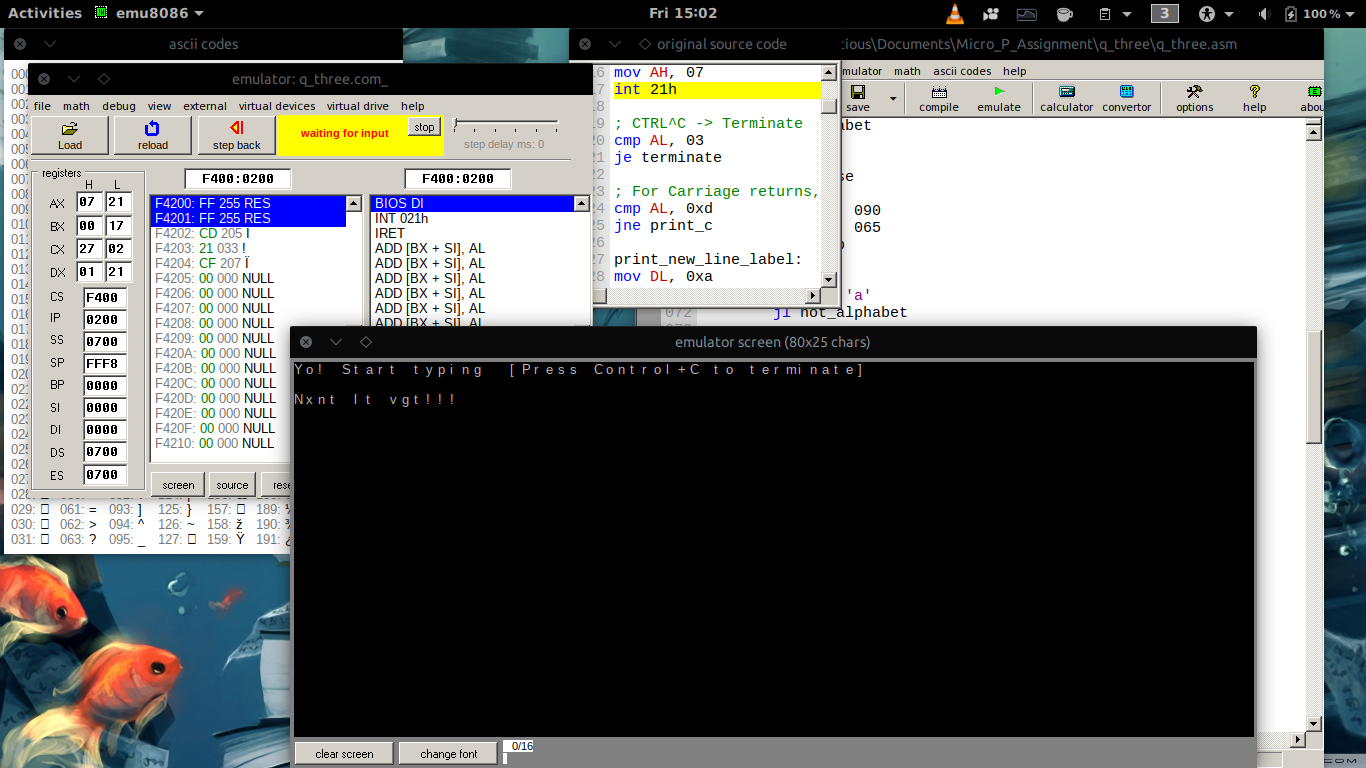
\includegraphics[width=12cm]{q_three/Q3_printing_make_me_cry!!!.png}
	\centering
	\caption{A screenshot of the output from running script \ref{sketch 3}. \textbf{The output of the input "make me cry!!!"}}
\end{figure}

\end{document}


